In this section, the team will describe all of the various artifacts that the team will generate and maintain during the project lifecycle.

\subsection{Project Charter}
The purpose of the Project Charter is to lay out an idea of what the project will be about and what the finished product will be. The Project Charter will be posted on GitHub with the rest of the team's documents.

\subsection{Product Backlog}
The team will be using scrumdesk.com to keep track of the amount of hours worked on certain aspects of the project. The team will discuss the backlog requirements during meetings and vote on times to required to complete the backlog item. The team will keep in touch with the stakeholders to decide backlog prioritization.

\subsection{Sprint Planning}
Sprint planning will be done in person and recorded in journals on the third week on a Thursday.

\subsubsection{Sprint Goal}
The sprint goal will be recorded in team members journals and will be recorded in the future on scrumdesk.com.

\subsubsection{Sprint Backlog}
The team will be using scrumdesk.com to keep track of the amount of hours worked on certain aspects of the project

\subsubsection{Task Breakdown}
Task breakdown is all recorded in journals during meeting times.

\subsection{Sprint Burndown Charts}
Sprint Burndown Chart. Culmination of hours of each day.

\begin{figure}[h!]
    \centering
    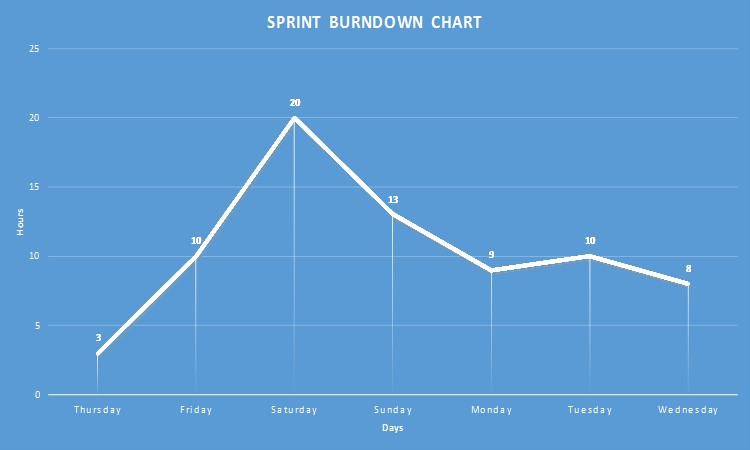
\includegraphics[width=0.5\textwidth]{images/test_image}
    \caption{Sprint burndown chart}
\end{figure}

\subsection{Sprint Retrospective}
The team will hold a retrospective meeting, write down information in their journal, and a presentation will be created every Thursday before the retrospective presentation on Friday.

\subsection{Individual Status Reports}
Individual Status Reports are done when the professor decides to check the engineering notebooks.

\subsection{Engineering Notebooks}
Engineering Notebooks are maintained by each team member. The purpose is to log information discussed in meetings and personal ideas about the project.

\subsection{Closeout Materials}
The team will deliver the project charter, the SRS, the source code, and binaries to the stakeholders when the project is finished. The user manuals will be distributed to the smart hospital team when the product launches.

\subsubsection{System Prototype}
Protoypes will be stored on GitHub and presented to stakeholders during the appropiate times.

\subsubsection{Project Poster}
The project poster will be debated at a later time.

\subsubsection{Web Page}
The web page will be stored on a UT Arlington server and created at a later time. The purpose will be to provide information about the creation process.

\subsubsection{Demo Video}
The demo video will be made at a later time.

\subsubsection{Source Code}
The source code will be maintained on GitHub.

\subsubsection{Source Code Documentation}
The source code documentation will be stored on GitHub and provide development comments and reference informaiton.

\subsubsection{Installation Scripts}
The installation scripts will be made at a later time.

\subsubsection{User Manual}
The user manuals will be distributed to the smart hospital team when the product launches. The manuals will be availble on the website after the product launches.